\minitoc

\vfill

In the previous chapter (Chapter~\ref{chap::semantic_evaluation}), we developped a hierchical and modular taxonomy of errors for the overhead modeling case.
Based on this taxonomy, and depending on the particular needs, specific error labels are extracted and considered during the quality evaluation.\\
In this chapter, we present the second part of our proposed approach.
It is based on formulating the problem as a supervized classification one.
Issues related to the latter are detailed in Section~\ref{sec::learned_evaluation::classification}.
Next, Section~\ref{sec::learned_evaluation::baseline} presents in details the baseline of features extracted out of building \gls{acr::3d} models.
Third and last, advanced features are discussed in Section~\ref{sec::learned_evaluation::richer_features}.
These are proposed to better model defect predictions.

\clearpage

\section{Quality evaluation as classification}
    \label{sec::learned_evaluation::classification}
    In order to satisfy the \textbf{large-scale} condition imposed at Subsection~\ref{subsec::introduction::contributions::positioning}, we propose to formulate the problem as a supervized learning one.
    Errors are considered as labels while features are computed so as to describe the observed buildings.
    Actually, as a first approach, the existence of all errors is predicted at the building level, even for \texttt{Facet Errors} labels\footnote{These errors are, in fact, by definition more local.}.
    Determining which facet is affected by an error is a much more challenging problem than the previous one.
    That is why the facet level prediction of errors is not explored in this work.
    The goal is, instead, to test the feasibility of the learning approach.\\

    Errors are predicted based on learned statistical characteristics of the evaluated models.
    The learned approach is usually used to take care of highly semantic tasks, such as ours, that are otherwise hard to process using engineered metrics \addref.\\
    Provided an initial manual annotation effort, the prediction phase is fully automatic, as will be proved by experimental results in Chapter~\ref{chap::experiments}.
    In order for this approach to be scalable at large scales, and hence verify the second constraint in Subsection~\ref{subsec::introduction::contributions::positioning} which is \textbf{automation}, prediction results should be stable enough independently of the urban scene.
    This is fully studied in Chapter~\ref{chap::more_experiments}.\\

    Two aspects should be discussed to in order to apply this approach to the building \gls{acr::3d} model quality evaluation.
    First, as seen in Section~\ref{sec::semantic_evaluation::label_extraction}, the parametric nature of the taxonomy leads to a varying set of labels.
    For this purpose, we describe in Subsection~\ref{subsec::learned_evaluation::classification::different_porblems} the different classification problems depending on the evaluation parameters.
    Second, the feature extraction procedure should also be compliant with the \textbf{large-scale} objective set beforehand.
    This aspect and more are detailed in Section~\ref{subsec::learned_evaluation::classification::feature_extraction}.
    Third, the classifier should be able to handle the heterogeneity of the feature vector and must adapt to different input vectors types and sizes.
    The choice of classifiers is, hence, discussed in Subsection~\ref{subsec::learned_evaluation::classification::classifiers}.

    \subsection{Different classification problems}
        \label{subsec::learned_evaluation::classification::different_porblems}
        The nature of the different classification problems are presented in Table~\ref{tab::classification_problems} depending on the three evaluation parameters defined in Subsection~\ref{sec::semantic_evaluation::label_extraction}.\\

        \begin{table}[htbp]
            \small
            \begin{tabular}{c c c x{11cm}}
                \toprule
                \textbf{\gls{acr::efin}} & \textbf{\gls{acr::elod}} & \textbf{exclusivity} & \textbf{Classification output}\\
                \midrule
                1 & --- & --- & $binary(\texttt{Valid}, \texttt{Erroneous})$\\
                2 & \gls{acr::lod}-1 & --- & $binary(\texttt{Valid}, \texttt{Building Errors})$\\
                2 & \gls{acr::lod}-2 & \textsc{on} & $multi\_class(\texttt{Valid}, \texttt{Building Errors}, \texttt{Facet Errors})$\\
                2 & \gls{acr::lod}-2 & \textsc{off} & $multi\_label(\texttt{Building Errors}, \texttt{Facet Errors})$\\
                3 & \gls{acr::lod}-1 & \textsc{on} & $multi\_stage(\texttt{Valid}, \texttt{Building Errors})$\\
                3 & \gls{acr::lod}-2 & \textsc{on} & $multi\_stage(\texttt{Valid}, \texttt{Building Errors}, \texttt{Facet Errors})$\\
                3 & \gls{acr::lod}-1 & \textsc{off} & $multi\_label(\operatorname{children}(\texttt{Building Errors}))$\\
                3 & \gls{acr::lod}-2 & \textsc{off} & $multi\_label(\operatorname{children}(\texttt{Building Errors})\cup \operatorname{children}(\texttt{Facet Errors}))$\\
                \bottomrule
            \end{tabular}
            \caption{
                \label{tab::classification_problems}
                All possible classification problem types depending of the evaluation parameters:
                \textbf{\gls{acr::efin}}, \textbf{\gls{acr::elod}} and \textbf{exclusivity}.
            }
        \end{table}

        In Table~\ref{tab::classification_problems}, $multi\_class(l_1, l_2, \dots, l_c)$ (\textit{resp.} $multi\_label(l_1, l_2, \dots, l_c)$) corresponds to the multi-class (\textit{resp.} multi-label) setting.
        We note that:
        \begin{equation*}
            multi\_label(\texttt{Valid}, l_1, l_2, \dots, l_c) \equiv multi\_label(l_1, l_2, \dots, l_c).
        \end{equation*}
        $binary$ refers to the special case of $multi\_class$ where $c = 2$: \textit{i.e}
        \begin{equation*}
            binary(l_1, l_2) \equiv multi\_class(l_1, l_2)
        \end{equation*}
        Two consecutive classification problems can be concatenated in a hierchical multi-stage classification:
        depending on the class that is predicted in the first stage multi-class classifier, a second classification problem predicts the existence of some corresponding labels.
        This denoted by:
        \begin{equation*}
            multi\_stage(l_1, l_2, \dots, l_3) \equiv multi\_label(\operatorname{children}(multi\_class(l_1, l_2, \dots, l_3))).
        \end{equation*}
            
        \textbf{\gls{acr::efin}} = 1 level corresponds to the standard binary classification problem: \texttt{Valid} or \texttt{Erroneous}.
        At \textbf{\gls{acr::efin}} = 2, the \textbf{\gls{acr::elod}} can then take two values in the aerial reconstruction case: \gls{acr::lod}-1 or \gls{acr::lod}-2.
        If set at \gls{acr::lod}-1, it is a binary classification problem: \texttt{Valid} or \texttt{Building Errors}.
        For \gls{acr::lod}-2, if the \textbf{exclusivity} is on, it will be a multi-class problem: \texttt{Valid}, \texttt{Building Errors} or \texttt{Facet Errors}.
        If set off, it becomes a multi-label one with the same labels.
        At \textbf{\gls{acr::efin}} = 3 level, if the \textbf{exclusivity} is on, it is a 2-stage classification problem.
        In the first stage, a multi-class task\footnote{It is binary in the spcial case \gls{acr::elod} = \gls{acr::lod}-1, problem, like in the previous semantic degree.}
        predicts the error family, after which a second multi-label problem decides between the predicted error family children.
        If the \textbf{exclusivity} is off, it turns into one stage multi-label problem that predicts the existence of each atomic error corresponding to the chosen \gls{acr::elod}.
    
    \subsection{Feature extraction}
        \label{subsec::learned_evaluation::classification::feature_extraction}
        The proposed quality evaluation approach, being formulated as a supervized classification problem, requires extracting feature vectors describing characteristics of the evaluated model.
        This is possible through the use of the intrinsic properties of the building model, as well as comparisons with external data.\\
    
        Intrinsic feature extraction consists in make use of the geometric structure of the \gls{acr::3d} model.
        Equally, semantics, as well as building model meta-data, could be utilized for the purpose of intrinsically evaluating a model.
        This case corresponds to the minimal amount of information one can use for building model evaluation.
        In this case, we talk about self-evaluation of building models.
        Since we are considering all possible cases, especially automatically reconstructed building models, only the model geometry is guaranteed to be always available.\\
    
        Extrinsic feature extraction relies on comparing the model to an available external data.
        Obviously, high quality reference models are the best type of data to compare the evaluated model to.
        However, taking into consideration the \textbf{large-scale} objective that was fixed earlier (subsection~\ref{subsec::introduction::contributions::use}), this is not a viable solution.
        We rely then on more basic reference data such as remote sensing acquired data that are the basis of large-scale modeling of urban scenes.\\
        For instance, raw depth information can be used in quality evaluation.
        It can prove helpful in detecting geometric defects that are intrinsically of \gls{acr::3d} nature.
        This was illustrated in Figure~\ref{fig::fig}, as comparing the projected model to the orthoimage did not yield anything out of place, contrarily to the \gls{acr::dsm} comparison.
        Depth data can take multiple forms: unstructured point clouds, originating for instance from \gls{acr::lidar} sensors, or dense depth maps such as \gls{acr::dsm} for the overhead case.\\
        Optical images can also be employed in this framework.
        These provide complementary information such as edges (high frequencies, in general) and textures which are suited for inner defect detection as an example (\textit{cf.} Subfigure~\ref{subfig::fus_2d}).
        This type of data comes usually in two different shapes: oblique images or orthoimages.
    
    \subsection{Classifier choice}
        \label{subsec::learned_evaluation::classification::classifiers}
        The choice of classifiers shoud take into consideration the highly modular nature of the framework with multimodal features involving many parameters.
        Two classifiers where chosen in this study: \gls{acr::rf} and \gls{acr::svm}.
        Both were discussed at great length in Section~\ref{sec::state_of_the_art::mlpr}.
        Hereafter, we explain how each one is used in this setting.\\

        \subsubsection{\acrlong*{acr::rf}}
            \gls{acr::rf} classifiers is a natural choice in our case.
            As seen in Sub-subsection~\ref{subsubsec::state_of_the_art::mlpr::classifiers::rf}, this type of classifiers can manage a large number of features with different dynamics and coming from multiple modalities.
            In fact, the computed features could be geometric, image based or height based.
            Each one of these modalities can also be heterogeneous in terms of extracted value types, as will be discussed later in Section~\ref{sec::learned_evaluation::baseline}.
            Relying on their bagging property, a high number of trees is required to cover most of the feature space, while a limited tree depth is needed to avoid overfitting during training.
            While the multi-class case is natively taken into account by the \gls{acr::rf} classifier, the multi-label one requires adopting a one-vs-all approach so as to address each label separately.

        \subsubsection{\acrshort*{acr::svm}}
            \glspl{acr::svm} do not manage well enough heterogeneity in feature vectors.
            Moreover, only binary classification is inherently handled.
            However, it offers other advantages that are not met by \gls{acr::rf}.
            In fact, \glspl{acr::svm} can be useful when labels are not equally distributed in the training set.
            This is actually the case of some errors that are rare in our dataset: specifically the inaccurate topology ones (\textit{cf.} Subsection~\ref{subsec::experiments::datasets::stats}).
            This type of classifiers naturally encorporates kernels such as the ones presented later in Subsection~\ref{subsec::learned_evaluation::richer_features::graph}.
            Finally, it is also preferred when dealing with high dimensional feature vectors like those produced by \glspl{acr::scatnet} (\textit{cf.} Subsection~\ref{subsec::learned_evaluation::richer_features::image}).

\section{Feature baseline}
    \label{sec::learned_evaluation::baseline}
    Since there is no comparable work that studied the learned detection of errors defined in Chapter~\ref{chap::semantic_evaluation}, we propose a baseline for each one of the three modalities: geometric, height based and image based features.
    Attributes are kept simple so as to be used in most situations relying on generally available data.
    We avoid computing and comparing \gls{acr::3d} lines~\parencite{michelin2013quality}, correlation scores~\parencite{boudet2006supervised} or any \gls{acr::sfm} based metric~\parencite{kowdle2011active}.
    In addition of being very costly, these features are methodologically redundant with the \gls{acr::3d} modeling techniques.
    They are, hence, vulnerable to the same defects.
    Conversely, evaluation metrics used in the \gls{acr::3d} building reconstruction literature (\textit{e.g.}, \gls{acr::rmse}) are too weak for such a complex task.
    This will be proven later on in Section~\ref{sec::experiments::baseline_feature_analysis}.

    In Subsection~\ref{subsec::learned_evaluation::baseline::geometric}, we describe the used baseline for geometric features.
    Next, in Subsection~\ref{subsec::learned_evaluation::baseline::height}, height based features extraction is explained.
    We end with image based features in Subsection~\ref{subsec::learned_evaluation::baseline::image}.

    \subsection{Geometric features}
        \label{subsec::learned_evaluation::baseline::geometric}
        Given a building model \(\mathsf{M}\), the facet set is denoted by $\mathsf{F_M}$.
        $\forall (f, g) \in \mathsf{F_M} \times \mathsf{F_M} \; f \sim g$ correspond to facets $f$ and $g$ being adjacent: 
        \textit{i.e.}, they share a common edge. As the roof topology graph in~\parencite{verma20063d}, the input building model $\mathsf{M}$ can be seen as a facet (dual) graph:

        \begin{equation}
        	\label{eq::model_graph}
        	\mathsf{M} \triangleq \left(\mathsf{F_M}, \mathsf{E_M} \triangleq \left\{ \left\{f, g\right\} \subset \mathsf{F_M} : f \sim g \right\} \right).
        \end{equation}

        \begin{figure}[htbp]
            \centering
            \includestandalone[mode=buildnew, width=.75\textwidth]{figures/features/geometric}
            \caption{
                \label{fig::geometric_features}
                Computed geometric attributes represented on the dual graph, for facets $f$ and $g$.
                The green vector groups the node (facet) attributes while the blue one shows the edge features.
            }
        \end{figure}

        The dual graph is illustrated in Figure~\ref{fig::geometric_features}.
        For each facet $f \in \mathsf{F_M}$, we compute its degree (\textit{i.e.}, number of vertices; $f \mapsto d\left(f\right) \triangleq \left\lvert\left\{v : v\text{ is a vertex of }f\right\}\right\rvert$), its area $f \mapsto \mathscr{A}\left(f\right)$ and its circumference $f \mapsto \mathscr{C}\left(f\right)$.
        These are all geometric invariants with respect to $\mathbb{R}^3$ isometries, contrarily to facet centroids $\mathscr{G}\left(f\right)$ and normals $\vec{n}\left(f\right)$.
        This is countersteped by looking, for each graph edge $e=\left\{f, g\right\} \in \mathsf{E_M}$, for the distance between facet centroids $\left\{f, g\right\} \mapsto \left\lVert \mathscr{G}\left(f\right) - \mathscr{G}\left(g\right) \right\rVert$ and the angle formed by their normals $\left\{f, g\right\} \mapsto \arccos\left(\vec{n}\left(f\right) \cdot \vec{n}\left(g\right)\right)$.
        Statistical characteristics are then computed over building model facets using specific functions \(\chi\), like a histogram:        

        \begin{equation}
            \label{eq::histogram_extractor}
        	\chi = \chi^p_{\operatorname{histogram}}: l \mapsto \operatorname{histogram}(l, p),
        \end{equation}
        with $p$ standing for histogram parameters. A simpler option could be:
        \begin{equation}
            \label{eq::max_min_mean_med_extractor}
            \chi = \chi_{\max,\min,\operatorname{mean},\operatorname{med}}: l \mapsto \begin{bmatrix}
                \max(l)\\
                \min(l)\\
                \operatorname{mean}(l)\\
                \operatorname{median}(l)
            \end{bmatrix}.
        \end{equation}

        These features are designed for general topological errors.
        For instance, over-segmentation may result in small facet areas and small angles between their normals.
        Conversely, an undersegmented facet would have a large area.
        Later on, the importance of these features will be discussed in details based on experimental results.
        
        Each building $\mathsf{M}$ can consequently be characterized by a geometric feature vector that accounts for its geometric characteristics:

        \begin{equation}
        	\label{eq::geometric_features}
            v_{\text{geometry}}(\mathsf{M}) = \begin{bmatrix}
            	\chi \left(\left(d\left(f\right)\right)_{f \in \mathsf{F_M}}\right)\\
                \chi \left(\left(\mathscr{A}\left(f\right)\right)_{f \in \mathsf{F_M}}\right)\\
                \chi \left(\left(\mathscr{C}\left(f\right)\right)_{f \in \mathsf{F_M}}\right)\\
                \chi \left(\left( \left\lVert \mathscr{G}\left(f\right) - \mathscr{G}\left(g\right) \right\rVert \right)_{\left\{f, g\right\} \in \mathsf{E_M}}\right)\\
                \chi \left(\left( \arccos\left(\vec{n}\left(f\right) \cdot \vec{n}\left(g\right)\right) \right)_{\left\{f, g\right\} \in \mathsf{E_M}}\right)
            \end{bmatrix}.
        \end{equation}

        Additionally to individual facet statistics, regularity is taken into account by looking into adjacent graph nodes as in~\parencite{zhou20102}.
        Such features express a limited  part of structural information.
        Dealing with this type of information implies graph comparisons which are not a genuinely simple task to achieve.
        Since our objective is to build a baseline, this approach has not yet been considered.

    \subsection{Height based features}
        \label{subsec::learned_evaluation::baseline::height}
        Regarding this modality, raw depth information is provided, for a building model \(\mathsf{M}\), by a \gls{acr::dsm} as a \gls{acr::2d} height grid that is cropped to fit the building footprint: $dsm \in \mathbb{R}^{w_{\mathsf{M}} \times h_{\mathsf{M}}}$\footnote{\label{note::w_h}\(w_{\mathsf{M}}\) (\textit{resp.} \(h_{\mathsf{M}}\)) is the grid width (\textit{resp.} height) and is determined by the size of the building and the resolution of the \gls{acr::dsm}.}.
        This type of reference data must date back to the same time where the building models where produced.
        Otherwise a lot of defects will result simply from change in the scenery.\\
        
        \begin{figure}[htpb]
            \centering
            \includestandalone[width=\textwidth, mode=buildnew]{figures/features/height_based}
            \caption{
                \label{fig::height_based_features}
                Height-based features computed from the \gls{acr::dsm} residuals using histograms.
            }
        \end{figure}

        The \gls{acr::dsm} is compared to the model height~\parencite{bredif20073d,zebedin2008fusion}.
        The latter is inferred from its facets plane equations.
        It is rasterized into an grid structure $alt_{\mathsf{M}} \in \mathbb{R}^{w_{\mathsf{M}} \times h_{\mathsf{M}}}$ using the same spatial resolution as $dsm_{\mathsf{M}}$.
        The difference between the two height grids provides a discrepancy map as shown in Subfigure~\ref{subfig::residuals}).
        A baseline approach is herein proposed relying on the statistics of pixel values computed using the $\chi$ functions (\textit{cf.} Figure~\ref{fig::height_based_features}).\\

        \begin{equation}
            \label{eq::height_based_features}
            v_{\text{height}}\left(\mathsf{M}\right) = \chi \left( dsm_{\mathsf{M}} - alt_{\mathsf{M}} \right).
        \end{equation}

        The histogram could actually be computed for the building alone without taking into account the terrain arround it.
        However, since reference data is unavailable, cropping out the terrain height values implies that the building model footrpint is flawless, which is not the case.
        As a consequence, the heigth discrepancies around the building model are also computed in order to provide some information on the footprint shape, and hence detect \texttt{BIT} or \texttt{BIB} errors.\\

        Equation~\ref{eq::height_based_features} summarizes how building height-based features are computed.
        Different from a \gls{acr::rmse}~\parencite{lafarge2012creating,poullis2013framework}, the histogram captures the discrepancy distribution, which is particularly helpful in detecting undersegmentation defects or geometric imprecision.
        However, as for the previous geometric attributes, the grid structure information coming from the model is lost.
        Errors cannot be spatialized and linked to a specific facet.

    \subsection{Image based features}
        \label{subsec::learned_evaluation::baseline::image}
        The framework is general enough to encompass both orthorectified images and oblique ones.
        For now, we rely only on more accessible orthorectified images, eventhough they can be riddled with artifacts.
        In an ideal scenario, using oriented images is better for edge verification (as already shown in~\parencite{michelin2013quality}) as orthoimages are a byproduct of earlier ones.
        However, in practice, oblique imagery would give rise to other issues, especially, registration problems.\\

        We aim to benefit from the high frequencies in Very High Spatial Resolution optical images.
        Building edges, like any image edge, correspond to sharp discontinuities in images~\parencite{ortner2007building}.
        The latter are detected using gradient filters on images.
        Gradient based features are advantageous compared to any radiometry based ones.
        This is due to the fact that the latter are much less invariant to changes in the than the first ones.
        Indeed, classic Computer Vision techniques rely on gradient based features:~\textcite{lowe2004distinctive,dalal2005histograms}.
        This is adequate to our case where models and images are part of large heterogeneous datasets.\\
        
        We apply this to our context by comparing building model edges to local image gradients.
        We start by projecting building models in the nadir direction.
        For each facet \(f \in \mathsf{F_M}\), this operation takes into account occlusions and results in:
        \begin{description}
            \item[A \gls{acr::2d} polygon:] If the facet is not vertical (\textit{i.e.} \(\vec{n}(f) \cdot \vec{z} \neq 0\)) and not completly occluded by other facets;
            \item[A segment:] If the facet is vertical (\textit{i.e.} \(\vec{n}(f) \cdot \vec{z} = 0\));
            \item[An empty polygon:] If the facet is completly occluded by other facets.
        \end{description}
        The last two cases are filtered out and the final projection consists in a set of polygons forming a partition of the building footprint denoted:
        \begin{equation}
            \label{eq::facet_projections}
            \mathsf{F_M}^q \triangleq \{q(f): f \in \mathsf{F_M}\}
        \end{equation}
        where:
        \begin{description}
            \item[\(q\)] is the function that yields the projection of a facet if it is a polygon or an empty polygon othewise.
        \end{description}

        This projection is compared with a corresponding orthorectified image \(I_{\mathsf{M}} \in \mathbb{R}^{w_{\mathsf{M}} \times h_{\mathsf{M}} \times 3}\) as shown in Subfigure~\ref{subfig::model_nadir_projection}.
        For each facet projection, we isolate an edge \(s\) (Figure~\ref{subfig::segment_gradient_collinearity}).
        In an ideal setting, gradients computed at pixels $g \in I_{\mathsf{M}}$ that intersect $s$ need to be collinear with its normal $\vec{n}(s)$.
        In consequence, applying the one of the statistics functions $\chi$ defined in Equations~\ref{eq::max_min_mean_med_extractor} or~\ref{eq::histogram_extractor}, we compute the distribution of the cosine similarity between the local gradient and the normal all along that $s$:
        
        \begin{equation}
            \label{eq::corr_seg}
            \mathsf{D}_{\chi}(s, I_{\mathsf{M}}) \triangleq \chi \left( \left(\frac{\nabla I_{\mathsf{M}}\left(g\right) \cdot \vec{n}(s)}{\left\rVert \nabla I_{\mathsf{M}}\left(g\right)\right\rVert}\right)_{\substack{g \in I_{\mathsf{M}} \\ g \cap s \neq \emptyset}} \right).
        \end{equation}

        \begin{figure}[htpb]
            \begin{center}
                \floatbox{figure}{
                    \begin{subfloatrow}[2]
                        \ffigbox[\FBwidth]{
                            \caption{
                                Model facets (each represented by a specific color) are nadir projected onto the orthoimage.
                            }\label{subfig::model_nadir_projection}
                            }			
                            {
                                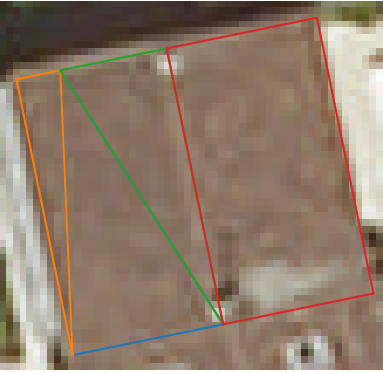
\includegraphics[width=.45\textwidth]{images/features/image/nadir_superposition}
                            }
                        \quad
                        \ffigbox[\FBwidth]{
                                \caption{Local gradients (in purple), on intersecting pixels (in green), are compared to the edge (in red) normal (in black).}
                                \label{subfig::segment_gradient_collinearity}
                            }
                            {\includestandalone[mode=buildnew, width=.45\textwidth]{figures/features/radiometric_features}
                        }
                    \end{subfloatrow}
                }{
                    \caption{Illustration of how features are derived from optical images.}\label{fig::image_based}
                }
            \end{center}
        \end{figure}

        For each polygon \(f^q \in \mathsf{F_M}^q\), the distributions over all its edges\footnote{The empty polygons are ignored as they have no edges.} \(s \in f^q\)\footnote{This is abuse of notation.} are stacked to yield a distribution over the whole projected facet.
        In the case of histograms $\chi^p_{\operatorname{histogram}}$ with the same parameters \(p\) (and thus the same bins), it is equivalent to summing out the previous vectors $\mathsf{D}_{\chi^p_{\operatorname{histogram}}}(s, I_{\mathsf{M}})$.
        In order to take into account the variability of segment dimensions, this sum is normalized by segment lengths.\\
        \begin{equation}
            \label{eq::corr_fac}
            D_{\chi^p_{\operatorname{histogram}}}\left(f^q, I_{\mathsf{M}}\right) \triangleq \sum_{s \in q\left(f\right)} \left\rVert s \right\lVert \cdot \mathsf{D}_{\chi^p_{\operatorname{histogram}}}(s, I_{\mathsf{M}}).
        \end{equation}

        The same can be done over all facets of a building $\mathsf{M}$.
        The weights are added in order to take into account the geometry heterogeneity.
        The gradient to normal comparison is similar to the \gls{acr::3d} data fitting term formulated in~\parencite{li2016manhattan}.
        Once again, the model structure is partially lost when simply summing histograms over all segments.

        \begin{equation}
            \label{eq::corr_bul}
            v_{\text{image}}\left(\mathsf{M}\right) = D_{\chi^p_{\operatorname{histogram}}}\left(\mathsf{M}, I_{\mathsf{M}}\right) \triangleq \sum_{f^q \in \mathsf{F_M}^q} \mathscr{A}\left(f^q\right) \cdot \mathsf{D}_{\chi^p_{\operatorname{histogram}}}(f^q, I_{\mathsf{M}}).
        \end{equation}
        
        These image-based attributes are helpful for precision error detection.
        As example, facet imprecise borders can be detected as local gradients direction will be expected to differ greatly from the inaccurate edge.
        It can also be detrimental in under-segmentation detection as colors can change considerably from one facet or one building to another inducing an gradient orthogonal to edge normals.

\section{Advanced features}
    \label{sec::learned_evaluation::richer_features}
    The last section presented features that are by construction taken to be as simple as possible.
    The goal was to test the feasibility of the learned quality evaluation approach.
    This is discussed in length in Subsection~\ref{sec::experiments::baseline_feature_analysis} and Sections~\ref{sec::more_experiments::finesse} and~\ref{sec::more_experiments::scalability}.\\

    This section presents features that better exploits structural information of the input models that were missed by the baseline.
    In the previous section, we identifed two types of instances from which features are extacted: graph-like and image-like data.
    Advanced graph based feature extractors are proposed in Subsection~\ref{subsec::learned_evaluation::richer_features::graph}.
    For images-like structures, better attributes are also presented in the next Subsection~\ref{subsec::learned_evaluation::richer_features::image}.

    \subsection{Graph kernels}
        \label{subsec::learned_evaluation::richer_features::graph}
        In Subsection~\ref{subsubsec::state_of_the_art::mlpr::feature_extraction::graph_classification}, were discussed some kernels that can describe adequately graphs.
        The geometric baseline features we provided in Subsection~\ref{subsec::learned_evaluation::baseline::geometric}, more precisely in Equation~\ref{eq::geometric_features}, could actually be seen as a concatenation of the basic feature maps from Equations~\ref{eq::feature_node_graph} and~\ref{eq::feature_edge_graph}.
        This corresponds, in fact, to the basic kernel in Equation~\ref{eq::feature_graph_kernel_sum}.\\

        The biggest disadvantage of this basic kernel is its disregard towards the structural information stored in the graph.
        That is why we propose to use the other kernels that are presented in Subsection~\ref{subsubsec::state_of_the_art::mlpr::feature_extraction::graph_classification}.
        None of these kernels takes into account edge attributes.
        This is actually not an issue as both the edge attributes of the facet graph (\textit{cf.} Equation~\ref{eq::model_graph}) are in fact a function of node attributes: centroid \(f \mapsto \mathscr{G}\left(f\right)\) and normal \(f \mapsto \vec{n}\left(f\right)\).
        Some of these kernels do not utilize the node attributes either as they take only account of the structure of the graph.\\

        Face normals are unit vectors with coefficients in the interval \([0, 1]\), while centroids are free to be roam in \(\mathbb{R}^3\).
        From a global standpoint, each one of the face geometric features have a specific dynammic.
        As a consequence, taking all these attributes into account by one graph kernel is going to raise some issues.
        One possible solution is to normalize all geometric features, concatenate them and associate the resulting node attribute vectors to one graph.
        We preferred instead to isolate each geometric feature in a specific graph.
        All graphs would share the same structure but each one takes as node attributes a type of geometric features.
        This results in three graphs.
        The first takes the face normals \(f \mapsto \vec{n}\left(f\right)\) as node attributes.
        The second graph has its nodes assigned face centroids \(f \mapsto \mathscr{G}\left(f\right)\).
        The last one has a composite vector
        \begin{equation*}
            f \mapsto \begin{bmatrix}
                d\left(f\right)\\
                \mathscr{A}\left(f\right)\\
                \mathscr{C}\left(f\right)            
            \end{bmatrix}
        \end{equation*} as node attributes.
        The degree, area and circumference, contrarily to the normal and centroid, of facets where inconsequential in error predictions according to the feature importances that were computed when training \glspl{acr::rf}.
        This explains why these were grouped into one vector in contrast with the other two features.\\

        Each graph can take multiple types of kernels.
        We use the kernels described in Sub-subsection~\ref{subsubsec::state_of_the_art::mlpr::feature_extraction::graph_classification}.
        Since all graphs share the same structure, kernels that ignore node attributes would yield the same results, no matter which node attribute is used.
        There are two such kernels: the random walk kernel and the \gls{acr::svm} \(\vartheta\) kernel.
        We also experimented with three other types of kernels: the Multiscale Laplacian kernel, the propagation kernel and the graph hopper kernel.
        The latter depends on the choice of the base kernel which compares node attributes.
        The \gls{acr::rbf} was briefly experimented and did not yield desirable results.
        Two alternatives were utilized:
        \begin{description}
            \item[Linear kernel:] As shown in Equation~\ref{eq::linear_kernel}, this is the most simple choice;
            \item[Brownian bridge kernel:] This base kernel was originally proposed for the Shortest Path kernel~\parencite{borgwardt2005shortest} and is also valid for its scalable derivation.
        \end{description}
        This results, in total, in \begin{equation*}
            \underbrace{2}_{\substack{\text{kernels ignoring}\\\text{ node attributes}}} + \underbrace{3}_{\substack{\text{attributed}\\\text{graphs}}} \times \left(\underbrace{2}_{\substack{\text{Multiscale Laplacian \&}\\\text{Propagation}}} + \underbrace{1}_{\text{Graph hopper}} \times \underbrace{2}_{\substack{\text{base}\\\text{kernels}}}\right) = 14
        \end{equation*} graph kernels.
        These are aggregated into one kernel using a linear combination.
        This is possible thanks to \gls{acr::mkl} as explained earlier in Sub-subsection~\ref{subsubsec::state_of_the_art::mlpr::classifiers::svm}.
        Other types of kernels were briefly experimented with, namely the Lov\'asz \(\vartheta\), Graphlet Sampling, Subgraph Matching and Shortest Path kernels.
        However, they did not yield any valuable results and most of the time failed numerically.
        
    \subsection{\acrshort*{acr::scatnet} feature extractor}
        \label{subsec::learned_evaluation::richer_features::image}
        \glspl{acr::cnn} have proven to be the standard feature extractors in image classification.
        However, they require a great load of images in order to learn good enough representations.
        This is not our case as explained later in Subsection~\ref{subsec::experiments::datasets::stats}.
        As a consequence, we choose instead to use \glspl{acr::scatnet} which mimic classical \glspl{acr::cnn} and can yield good image representations in an unlearned manner as shown in Sub-subsection~\ref{subsubsec::state_of_the_art::mlpr::feature_extraction::scatnet}.

        \subsubsection{Height based features}
            Discrepancies between the \gls{acr::3d} model extracted height map and the \gls{acr::dsm} manifest in textures in computed residuals (\textit{cf.} Figure~\ref{subfig::residuals}).
            As a matter of fact, \glspl{acr::scatnet} can handle very well texture discrimination as proven theoretically by~\textcite{mallat2012group} and experimentally by~\textcite{bruna2013invariant,sifre2013rotation}.
            In addition, theoretically the height data can be fed directly to a \gls{acr::scatnet} without requiring any normalization or preprocessing since, by construction, they can admit any type of \gls{acr::2d} signal\footnote{There are other versions of \glspl{acr::scatnet} taking one dimensional signals~\parencite{anden2014deep} or even graphs~\parencite{eickenberg2018solid}.}.
            This explains why \glspl{acr::scatnet} were chosen as a height based feature extractor.\\

            From a practical standpoint, the residuals computed as in Subsection~\ref{subsec::learned_evaluation::baseline::height} come as images in different sizes \(w_{\mathsf{M}} \times h_{\mathsf{M}}\)\cref{note::w_h} depending on the input model.
            Consequently, concatenating \gls{acr::scatnet} coefficients into a single vector is going to result in variable feature vector dimensions.
            One solution is to resize all images to a certain fixed size beforehand.
            However, this solution was quickly ruled out based on few experiments.
            In fact, aside from the fact that this process either looses valuable structural informations or adds undesired blur, it completly deforms the input signal as the \(\frac{w}{h}\) ratio is not guaranteed to constant for all inputs resulting in squashed or elongated image.
            Moreover, since \glspl{acr::scatnet} yields a great deal of coefficients that can easily surpass the number of training instances which hinders the learning ability of any classifier.
            As a consequence, we propose to add a function to help extract meaningful feature vectors with the same length.\\

            Suppose we have a function \(\chi: \mathbb{R}^{w_1 \times d_1} \rightarrow \mathbb{R}^d\) such as the ones presented in Equations~\ref{eq::histogram_extractor} and~\ref{eq::max_min_mean_med_extractor} which has the same output dimension no matter the input size \(w_1 \times d_1\).
            It can be applied on the output of each scattering output \(S_l[dsm - alt](\bullet, p)\):
            \begin{equation}
                \label{eq::reduced_scattering}
                \chi \left(S_m[dsm_{\mathsf{M}} - alt_{\mathsf{M}}]\left(\bullet, p_m\right)\right) \in \mathbb{R}^d.
            \end{equation}
            where:
            \begin{description}
                \item[\(l\)] is the scattering output layer;
                \item[\(p_m\)] is a valid path at layer \(l\) (\textit{cf.} Equation~\ref{eq::scatter_second}). 
            \end{description}
            
            The resulting coefficients defined in Equation~\ref{eq::reduced_scattering} can be concatenated for all \(n_S\) scattering paths to form a feature vector:
            \begin{equation}
                \label{eq::scatnet_height_based_features}
                v_{\text{scattered height}}\left(\mathsf{M}\right) = \begin{bmatrix}
                    \chi \left(S_0[dsm_{\mathsf{M}} - alt_{\mathsf{M}}]\left(\bullet\right)\right)\\
                    \vdots\\
                    \chi \left(S_1[dsm_{\mathsf{M}} - alt_{\mathsf{M}}]\left(\bullet, i_1, \theta_1\right)\right)\\
                    \vdots\\
                    \chi \left(S_2[dsm_{\mathsf{M}} - alt_{\mathsf{M}}]\left(\bullet, i_1, \theta_1, i_2, \theta_2, \xi_2\right)\right)\\
                    \vdots\\
                    \chi \left(S_m[dsm_{\mathsf{M}} - alt_{\mathsf{M}}]\left(\bullet, p_m\right)\right)
                \end{bmatrix}_{
                    \substack{
                        i_1 \in \llbracket 1, I \rrbracket\\
                        \theta_1 \in \frac{\pi}{L} \cdot \llbracket 1, L \rrbracket\\
                        i_2 \in \llbracket i_1 + 1, I \rrbracket\\
                        \theta_2 \in \frac{\pi}{L} \cdot \llbracket 1, L \rrbracket\\
                        \xi_2 \in \llbracket 1, \lfloor\log_2(L)\rfloor \rrbracket\\
                        \vdots\\
                        \lambda_m \in \Lambda_m
                    }
                } \in \mathbb{R}^{d \cdot n_S}.
            \end{equation}
            where:
            \begin{description}
                \item[\(\Lambda_m\)] is the space of all possible values of parameter \(\lambda_m\) at layer \(m\).
            \end{description}

            Regarding the \(\chi\) function it is taken herein as follows:
            \begin{equation}
                \label{eq::max_min_mean_med_std_extractor}
                \chi = \chi_{\max,\min,\operatorname{mean},\operatorname{med},\operatorname{std}}: l \mapsto \begin{bmatrix}
                    \max(l)\\
                    \min(l)\\
                    \operatorname{mean}(l)\\
                    \operatorname{median}(l)\\
                    \operatorname{std}(l)
                \end{bmatrix}.
            \end{equation}
            where:
            \begin{description}
                \item[\(\operatorname{std}(l)\)] computes the standard deviation over the tuple \(l\).
            \end{description}

        \subsubsection{Height based features}
            \glspl{acr::scatnet} seem then to be good choice for image based feature extractors.
            In fact, as shown in Subfigure~\ref{subfig::bus_2d}, image textures could be also useful for error detection.
            More importantly, as shown with baseline image based features (\textit{cf.} Subsection~\ref{subsec::learned_evaluation::baseline::image}), edges are key image attributes for comparing building models to orthoimages.
            Actually, \glspl{acr::scatnet} are well suited for edge detection as they use Morlet wavelets for convolution operations (\textit{cf.} Sub-subsection~\ref{subsubsec::state_of_the_art::mlpr::feature_extraction::scatnet}).
            These filters are adapted to edge detection~\parencite{zhang2007radon}, as depicted in Subfigure~\ref{subfig::morlet_filters}.\\

            In order to draw features comparing orthoimages to buildings models, we start first by rasterizing the borders of polygons \(f^q \in \mathsf{F_M}\) of the model into a grid structure mask:
            \begin{equation}
                \label{eq::borders_mask}
                Q_{\mathsf{M}} \triangleq \left(\mathbb{1}_{g_{i,j} \cap \left(\bigcup_{f^q \in \mathsf{F_M}}f^q\right)}\right)_{\substack{i \in \llbracket 1, w_\mathsf{M} \rrbracket\\j \in \llbracket 1, w_\mathsf{M} \rrbracket}}
            \end{equation}
            where:
            \begin{description}
                \item[\(g_{i,j}\):] is the rectangle\footnote{It is usually a square as both dimensions are equal.} representing the pixel at row \(i\) and column \(j\).
            \end{description}

            Two options are possible:
            \begin{description}
                \item[Deletion:] Pixels \(g\) in the corresponding orthoimage which are part of a polygon border (\textit{i.e.} \(Q_{\mathsf{M}}(g) = 1\)) are made black:
                        \begin{equation}
                            \label{eq::deletion_orthoimage}
                            I^{\text{dl}}_{\mathsf{M}} \triangleq I_{\mathsf{M}} \odot \left(\begin{bmatrix}
                                1 & 1 & \dots & 1\\
                                1 & 1 & \dots & 1\\
                                \vdots & \vdots & \ddots & 1\\
                                1 & 1 & \dots & 1\\
                            \end{bmatrix} - Q_{\mathsf{M}}^{\otimes 3}\right),
                        \end{equation}
                        where:
                        \begin{description}
                            \item[\(Q_{\mathsf{M}}^{\otimes 3} = Q_{\mathsf{M}} \otimes Q_{\mathsf{M}} \otimes Q_{\mathsf{M}}\)] is the tensor obtained by stacking in depth thee copies of the same matrix \(Q_{\mathsf{M}}\);
                            \item[\(A \odot B  = \left(A_{ij} \cdot B_{ij} \right)_{ij}\)] denotes the Hadamard/Schur product of any two matrices \(A\) and \(B\).
                        \end{description}
                \item[Channel:] The mask \(Q_{\mathsf{M}}\) is simply added to the orthoimage as a fourth channel:
                        \begin{equation}
                            \label{eq::channel_orthoimage}
                            I^{\text{ch}}_{\mathsf{M}} \triangleq I_{\mathsf{M}} \otimes Q_{\mathsf{M}}.
                        \end{equation}
            \end{description}
            The first situation corresponds to an early fusion scheme while the second represent a late fusion case.
            Both settings are experimented with and compared later in Subsection~\ref{subsec::more_experiments::richer_features::scatnet_baseline}.\\

            Now we can apply the \gls{acr::scatnet} on any of the previously defined images.
            We apply then the same post-processing to yield feature vectors with the same dimensions \(d \cdot n_S\):

            \begin{description}
                \item[Deletion:]
                        \begin{equation}
                            \label{eq::deletion_scanetg_image_based_features}
                            v^{\text{dl}}_{\text{scattered image}}\left(\mathsf{M}\right) \triangleq \begin{bmatrix}
                                \chi \left(S_0[I^{\text{dl}}_{\mathsf{M}}]\left(\bullet\right)\right)\\
                                \vdots\\
                                \chi \left(S_1[I^{\text{dl}}_{\mathsf{M}}]\left(\bullet, i_1, \theta_1\right)\right)\\
                                \vdots\\
                                \chi \left(S_2[I^{\text{dl}}_{\mathsf{M}}]\left(\bullet, i_1, \theta_1, i_2, \theta_2, \xi_2\right)\right)\\
                                \vdots\\
                                \chi \left(S_m[I^{\text{dl}}_{\mathsf{M}}]\left(\bullet, p_m\right)\right)
                            \end{bmatrix}_{
                                \substack{
                                    i_1 \in \llbracket 1, I \rrbracket\\
                                    \theta_1 \in \frac{\pi}{L} \cdot \llbracket 1, L \rrbracket\\
                                    i_2 \in \llbracket i_1 + 1, I \rrbracket\\
                                    \theta_2 \in \frac{\pi}{L} \cdot \llbracket 1, L \rrbracket\\
                                    \xi_2 \in \llbracket 1, \lfloor\log_2(L)\rfloor \rrbracket\\
                                    \vdots\\
                                    \lambda_m \in \Lambda_m
                                }
                            }.
                        \end{equation}
                \item[Channel:]
                        \begin{equation}
                            \label{eq::channel_scatnet_image_based_features}
                            v^{\text{ch}}_{\text{scattered image}}\left(\mathsf{M}\right) \triangleq \begin{bmatrix}
                                \chi \left(S_0[I^{\text{ch}}_{\mathsf{M}}]\left(\bullet\right)\right)\\
                                \vdots\\
                                \chi \left(S_1[I^{\text{ch}}_{\mathsf{M}}]\left(\bullet, i_1, \theta_1\right)\right)\\
                                \vdots\\
                                \chi \left(S_2[I^{\text{ch}}_{\mathsf{M}}]\left(\bullet, i_1, \theta_1, i_2, \theta_2, \xi_2\right)\right)\\
                                \vdots\\
                                \chi \left(S_m[I^{\text{ch}}_{\mathsf{M}}]\left(\bullet, p_m\right)\right)
                            \end{bmatrix}_{
                                \substack{
                                    i_1 \in \llbracket 1, I \rrbracket\\
                                    \theta_1 \in \frac{\pi}{L} \cdot \llbracket 1, L \rrbracket\\
                                    i_2 \in \llbracket i_1 + 1, I \rrbracket\\
                                    \theta_2 \in \frac{\pi}{L} \cdot \llbracket 1, L \rrbracket\\
                                    \xi_2 \in \llbracket 1, \lfloor\log_2(L)\rfloor \rrbracket\\
                                    \vdots\\
                                    \lambda_m \in \Lambda_m
                                }
                            }.
                        \end{equation}
            \end{description}
